\documentclass[12pt, landscape]{article}
\usepackage[scaled=0.92]{helvet}
\usepackage{multicol}
\usepackage{calc}
\usepackage{ifthen}
\usepackage[landscape]{geometry}
%\usepackage{hyperref}

\usepackage{newtxtext} 

%for strikeout
\usepackage{ulem}

%For editing parbox
\usepackage[table]{xcolor}
%For editing itemise margins, reduce iterm separaion and list separation
\usepackage{enumitem}
% For math
\usepackage{amsmath,amsthm,amsfonts,amssymb}

%For pictures / figures
\usepackage{color,graphicx,overpic}
\graphicspath{ {./images/} }

%\usepackage{newtxtext} 
%\usepackage{amssymb}
%\usepackage[table]{xcolor}
%\usepackage{vwcol}
%\usepackage{tikz}
%\usepackage{wrapfig}
%\usepackage{makecell}


% For Code Blocks
\usepackage{xcolor}
\usepackage{listings}

\lstdefinestyle{mystyle}{
	backgroundcolor=\color{gray!25!white},
	basicstyle=\scriptsize,
	numbers=none,    %or = none or left
	showstringspaces=false,
	breaklines=true,
	breakatwhitespace=false,                  
	captionpos=b,                    
	keepspaces=true,                                 
	numbersep=5pt,                  
	showspaces=false,                
	showtabs=false,                  
	tabsize=2,
 }
%Helpful:
%[linewidth = 1.0 \linewidth]
%\lstinline{}
% use \code{} for \lstinline with colorbox.
\newcommand{\code}[1]{\colorbox{gray!25!}{\lstinline|#1|}}
\lstset{style=mystyle}



%--------------------------- PACKAGES ABOVE --------------------------------------------------------------

\pdfinfo{
  /Title (Documentname.pdf)
  /Creator (Ger Teck)
  /Author (Ger Teck)
  /Subject ()
  /Keywords (tex)}

%% Margins for PAPER

% This sets page margins to .5 inch if using letter paper, and to 1cm
% if using A4 paper. (This probably isn't strictly necessary.)
% If using another size paper, use default 1cm margins.
\ifthenelse{\lengthtest { \paperwidth = 11in}}
	{ \geometry{top=.5in,left=.5in,right=.5in,bottom=.5in} }
	{\ifthenelse{ \lengthtest{ \paperwidth = 297mm}}
		{\geometry{top=1cm,left=1cm,right=1cm,bottom=1cm} }
		{\geometry{top=1cm,left=1cm,right=1cm,bottom=1cm} }
	}

% Turn off header and footer
\pagestyle{empty}

% for tight centres (less spacing)
\newenvironment{tightcenter}{%
  \setlength\topsep{0.5pt}
  \setlength\parskip{0.5pt}
  \begin{center}
}{%
  \end{center}
}

% Redefine section commands to use less space
\makeatletter
\renewcommand{\section}{\@startsection{section}{1}{0mm}%
                                {-1ex plus -.5ex minus -.2ex}%
                                {0.5ex plus .2ex}%x
                                {\normalfont\large\bfseries}}
\renewcommand{\subsection}{\@startsection{subsection}{2}{0.1mm}%
                                {-1explus -.5ex minus -.2ex}%
                                {0.5ex plus .2ex}%
                                {\normalfont\normalsize\bfseries}}
\renewcommand{\subsubsection}{\@startsection{subsubsection}{3}{0.1mm}%
                                {-1ex plus -.5ex minus -.2ex}%
                                {1ex plus .2ex}%
                                {\normalfont\small\bfseries}}
% change font
%\renewcommand{\familydefault}{\sfdefault}
%\renewcommand\rmdefault{\sfdefault}
\linespread{1.05}

\makeatother

% Define BibTeX command
\def\BibTeX{{\rm B\kern-.05em{\sc i\kern-.025em b}\kern-.08em
    T\kern-.1667em\lower.7ex\hbox{E}\kern-.125emX}}

% Don't print section numbers
\setcounter{secnumdepth}{0}

\setlength{\parindent}{0pt}
\setlength{\parskip}{0pt plus 0.5ex}

%% this changes all items (enumerate and itemize, reduce margins)
\setlength{\leftmargini}{0.5cm}
\setlength{\leftmarginii}{0.5cm}
\setlist[itemize,1]{leftmargin=2mm,labelindent=1mm,labelsep=1mm, itemsep = 1mm}
\setlist[itemize,2]{leftmargin=4mm,labelindent=1mm,labelsep=1mm, itemsep = 1mm}
%itemsep = 0mm
%\setlist{nosep}


%Watermark Top Right
\usepackage{atbegshi,picture}
\AtBeginShipout{\AtBeginShipoutUpperLeft{%
  \put(\dimexpr\paperwidth-1.2cm\relax, -1.2cm){\makebox[0pt][r]{\framebox{
\includegraphics[width = 0.3cm]{mountainbooks} Ger Teck}}}%
}}


% -------------------------------------------------------------------------------

% START OF DOCUMENT HERE

\begin{document}
\raggedright
\footnotesize
\begin{multicols*}{3}



% multicol parameters
% These lengths are set only within the two main columns
%\setlength{\columnseprule}{0.25pt}
\setlength{\premulticols}{1pt}
\setlength{\postmulticols}{1pt}
\setlength{\multicolsep}{1pt}
\setlength{\columnsep}{2pt}

%% DOCUMENT NAME HERE
\begin{center}
     \Large{\textbf{CS2030S Summary and Notes}} \\
\end{center}

% TABLE PACKAGE 
 \begin{center}
    \fbox{%
        \parbox{0.8\linewidth}{\centering \textcolor{black}{
            \\ \normalsize{AY22/23 Sem 2}}
            \\ {\footnotesize github.com/gerteck}
        }%
    }
  \end{center}

\section{Variables \& Types}
\subsection{Type Systems}
\begin{itemize}
	\item Dynamically typed: Variables can hold values of different types, checking of right type is done during execution of the program.
	\item \textbf{Statically typed}: [Java] Variables can only hold values of the same type. Type must be declared at compile time (CTT), type cannot be changed once assigned.
	\item \textbf{Strong vs. Weak Typing}: Strongly typed language enforces strict rules in type system to ensure type safety, to catch type errors during compile time rather than leaving to runtime. Weakly (Loosely) typed is more permissive in terms of type checking. 
	\item A variable is an abstraction! (of a name to some location in computer memory) \\
	\item \textbf{Primitive Types in Java:}

\begin{lstlisting} [linewidth = 1.0 \linewidth],
byte <: short <: int<: long <: float <: double
 char <: int
 boolean
\end{lstlisting}

	\item \textbf{Subtypes:}\\
 If S is a subtype of T, \code{S <: T }, we say that a piece of code written for variable of type \code{S} can be safely used on variables of type \code{T}. (LSP)
	\begin{itemize}
		\item Widening Type Conversion $\rightarrow$ e.g. type \code{S} being put into type \code{T} (Auto).
		\item \textbf{Narrowing Type Conversion} $\rightarrow$ requires typecasting (Error: Incompatible types / ClassCastException)
	\end{itemize}

	\item \textbf {Run Time Type (RTT) vs. Compile Time Type (CTT)}

\end{itemize}


\textbf{Range-based For Loops}
\begin{itemize}
	\item \code{for(x : collection)} or \code{for(T x : collection)}
	\item Works with any collection that implements \code{Iterable<U>} where $U$ is implicit-convertible to $T$, even if $T$ is a primitive type.
\end{itemize}

\subsection{Liskov Substitution Principle}
If \code{S <: T }, then 
\begin{itemize}
	\item Any property of \code{T} should be a property of \code{S}, including fields and methods. An object of type \code{T} can be replaced with \code{S} without changing some desirable property of the program.
	\item "Let $\phi(x)$ be a property provable about objects x of type T. Then $\phi(y)$ should be true for objects y of type S where S is a subtype of T." 
\end{itemize}



\section{OOP Principles}
\textbf{Abstraction, Encapsulation, Polymorphism and Inheritance. }
\subsubsection{Abstraction}
\begin{itemize}
	\item	Intention revealing, easy/simple to use and understand. Allows compartmentalized computation and effects. Hide how tasks are performed, and reduce repetition through code reuse. \\
	\item \textbf{Abstraction Barrier}: Implementer vs. Client
\end{itemize}

\subsubsection{Encapsulation}
\begin{itemize}
	\item Keeping all data and functions related to a composite data type together within an abstraction barrier.
	\item Composite Data Types - Class is a data type with a group of functions (methods), data (fields).
	\item \code{private} attributes, \code{public} methods. (Data hiding) Use constructors to initalize object and access private variables. \textbf{Ex. Constructor:}
\begin{lstlisting}
public Circle(Point p, double r){
	this.p = p;
	this.r = r;
\\this keyword used to refer to self / Object
}
\end{lstlisting}
	$\star$ Any reference variable that is not initialized will have the special reference value \code{null}. 
\subsubsection{Tell, Don't Ask}
	\item Avoid using unnecessary accessors (getters) and mutators (setters) as they break the abstraction barrier, [encapsulation]. Tell the object/class to do something, don't ask for details and do it yourself. 
	\item Encourage behaviour to be moved into an object to go with the data. \\
	\textbf{Static vs. Instance Methods and Fields}\\
	\item To associate method or field with class, we declare them with \code{static} keyword. We may also add \code{final} to indicate that value of field will not change, and \code{public} to indicate that field is accessible from outside the class.
	\item \code{main} method is entry point to Java program. \code{main} method takes in an array of strings as parameters. Defined as follows:
\begin{lstlisting}
public static void main(String[] args){
}
\end{lstlisting}
	\item use \code{import} to access classes from Java standard libraries.
\end{itemize}

\subsubsection{Inheritance}
\begin{itemize}
	\item "has-a" relationship:  $\rightarrow$ use composition (e.g. Circle has-a point as center)
	\item "is-a" relationship $\rightarrow$ \code{extends} (subtyping) \\
	$\star$ In Java, every class not extending another class inherits from the class Object implicitly. ("ancestor" of all classes), Object is at the root of the class hierarchy. 
	\item we use \code{super} to call the constructor of the superclass, to initialize (in example) its center and radius (since the child has no direct access to these fields that it inherited).
\begin{lstlisting}
class ColoredCircle extends Circle {
  private Color color;

  public ColoredCircle(Point center, double radius, Color color) {
    super(center, radius);  // call the parent's constructor
    this.color = color;
  }
}
\end{lstlisting}

	\item Inheritance tends to be overused, make sure inheritance preserves the meaning of subtyping.

\end{itemize}


\subsubsection{Polymorphism}
Changes how existing code behaves, without changing a single line existing of code.
\begin{itemize}
	\item  \textbf{Dynamic Binding} $\rightarrow$ method invoked is determined at run time RT (while possibilities [method signatures] determined at compile time CT). 
	\item \textbf{Method Overloading (static Polymorphism}: same method name, but \textbf{different parameter types/number of parameters}
	\item \textbf{Method Overriding (dynamic Polymorphism}: same \textbf{method signature}: (method name, type/number/order of parameters). Note method descriptor = method signature + return type. \\
	(ex. of polymorphism $\rightarrow$ overriding parent class method)
	\item Return type of overriding method can be subtype but not super type, or compiler will throw an error.
	\item Exceptions and return types are not part of function signature. 
	\item \code{Overridding Object::toString method}
\begin{lstlisting}
//Override annotation to help compiler help us
  @Override
  public String toString() {
      return "{ center: " + this.c + ", radius: " + this.r + " }";
  }
//center: (0.0, 0.0), radius: 4.0
\end{lstlisting}
	\item \code{private, static, final} methods cannot be overridden \\

\subsubsection{Method Invocation}
	Determine which non-static method to use through dynamic binding. During \textbf{compile time}, determine most specific method descriptor method to invoke (using \code{Type Information}. During \textbf{run time}, use \code{Objects} to determine binding.
	\item Class methods (\code{static} do not support dynamic binding (resolved statically) \\

\subsubsection{Abstract Classes}
	\item Cannot be instantiated. As long as one method is abstract, whole class is abstract.
	\item A concrete class cannot have abstract methods. \\
	
\subsubsection{Interface "can-do"}
	\item Interface is also a type and is declared as follows. As it models what an entity can do, name usually ends with -able suffix.
\begin{lstlisting}
interface GetAreable {
  	public abstract double getArea();
// public abstract fields r default, equiv to
	  double getArea();
}
abstract class Shape implements GetAreable { 
}
\end{lstlisting}
	\item For a concrete class to implement an interface, override all abstract methods \textbf{(*using same method signature)} from interface and provide implementation. Otherwise, the class becomes abstract.
	\item Note: A class can only extend from one superclass, but it can implement multiple interfaces. 
	\item Note: An interface can \code{extend} from one or more other interfaces, but an interface cannot extend from another class. (Neither can an interface \code{implements} other interfaces as it is abstract.
\end{itemize}

\subsection{Stack and Heap (Memory Model)}
	\textbf{Stack} is the region where all variables (including primitives and object references) are allocated in and stored. \\
	\textbf{Heap} is the region of memory where all objects are allocated in and stored, \\ ~\\
	\centerline{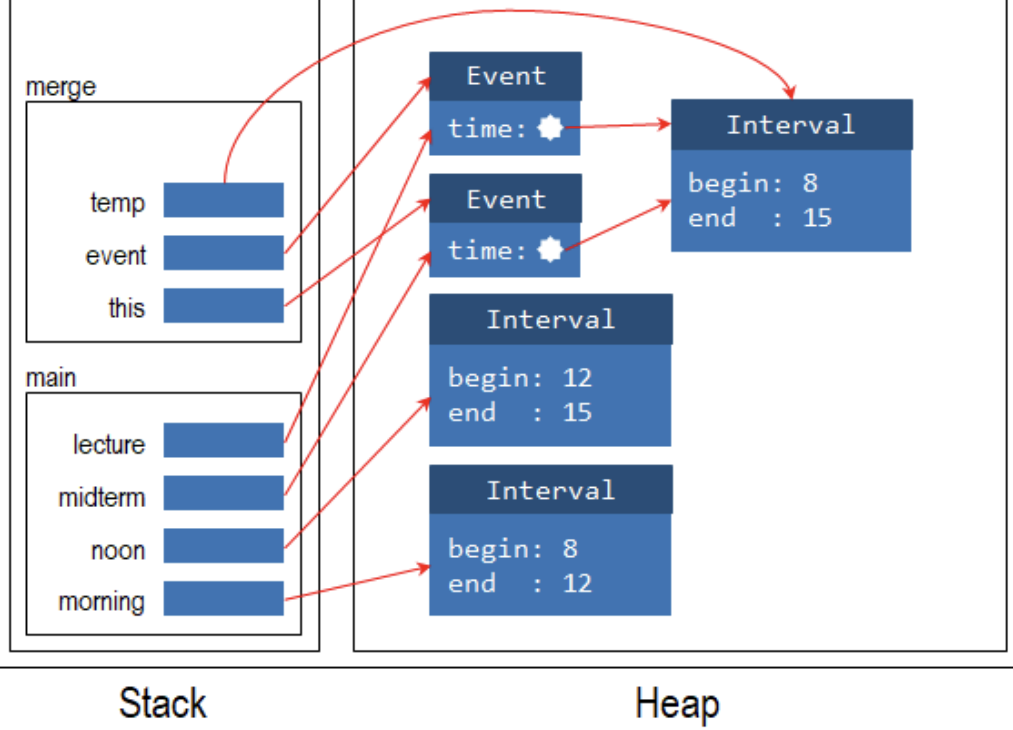
\includegraphics[width=0.5 \linewidth]{stackandheap}}
	\textbf{Stack frame of Primitives} Note radius value is primitive type instead of reference, we copy the value onto the stack. Java uses call by value for primitive types, and call by reference
 for objects. \\
\begin{itemize}
	\item	\code{this} reference is always placed on the stack when calling a non-static method 
	\item The memory allocated on the stack is deallocated when a method returns. The memory allocated on the heap, however, stays there as long as there is a reference to it. The JVM runs a garbage collector that checks for unreferenced objects on the heap and cleans up the memory automatically.
\end{itemize}

\section{Wrapper Class for Primitives}
"Making primitive types less primitive". A wrapper class is a class that encapsulates a type. 
\begin{lstlisting}
Integer i = new Integer(2); // = new Integer.valueOf(int a)
int j = i.intValue();
\end{lstlisting}
\begin{itemize}
	\item All wrapper class objects are immutable. Autoboxing $\rightarrow$ primitive value converted to instance of Wrapper class (\code{int}$\rightarrow$ \code{Integer}). Unboxing is the opposite type conversion.
	\item Wrapper classes incur cost of allocating memory for object and collecting garbage afterwards. Because they are immutable, new object must be created for update of value. (Inefficient)
\end{itemize}

\section{Modifiers}
\begin{itemize}
	\item In Order of Java modifiers:
\begin{lstlisting}
public protected private abstract default static sealed non-sealed final transient volatile synchronized native strictfp
\end{lstlisting}
	\item \code{private} $\rightarrow$ only within class, \code{public} $\rightarrow$ everywhere
	\item \code{default} $\rightarrow$ only within package, \code{protected} $\rightarrow$ within package or outside package through child class ~\\

	\item \code{final} variable $\rightarrow$ only assigned once (immutable)
	\item \code{final} class $\rightarrow$ cannot be inherited from
	\item \code{final} method $\rightarrow$ cannot be overridden

\end{itemize}

\section{Casting}
\begin{lstlisting}
// Circle <: Shape <: GetAreable
GetAreable findLargest(GetAreable[] array){...}
GetAreable ga = findLargest(circles);  // ok

Circle c1 = findLargest(circles); // error
Circle c2 = (Circle) findLargest(circles); // ok
\end{lstlisting}
\begin{itemize}
	\item In the snippet above, we can be sure (even prove) that the returned object from findLargest must have a run-time type of Circle since the input variable circles contains only Circle objects.
	\item Only cast when you can prove it is safe.
\end{itemize}

\section{Variance}
Variance of types refers to how the subtype relationship between complex types relates to the subtype relationship between components.
\begin{itemize}
\item Let $C(S)$ corresponds to some complex type based on type S. An array of type $S$ is a complex type. \\
We say a complex type is:
	\item \textbf{covariant} if  $S<: T$ implies $C(S)<: C(T)$
	\item \textbf{contravariant} if $S<: T$ implies $C(T)<: C(S)$
	\item \textbf{invariant} if it is neither covariant nor contravariant. \\ ~\\
Note:
	\item \textbf{Array is covariant in Java}. This means that, if $S<: T$ implies $S[]<: C[]$ \\
	By making array covariant, Java opens up the possibility of run-time erros without typecasting.	
\end{itemize}
\begin{lstlisting}
Integer[] intArray = new Integer[2] {
  new Integer(10), new Integer(20)
};
Object[] objArray;
objArray = intArray;
objArray[0] = "Hello!"; // <- compiles!

// But will lead to a runtime error, as we are 
// stuffing a string into an array of integers. (Heap Pollution)
\end{lstlisting}

\section{Exceptions}
\subsubsection{\code{try catch finally} blocks}
\begin{lstlisting}
try {
	new Circle(new Point(1,1), 0);
	// everything afterwards is skipped (r//= 0)
	System.out.println("This will not be reached");
} catch (IllegalCircleException e) {
	//runs if there is an exception
} finally {
	always runs
}
\end{lstlisting}
\begin{itemize}
	\item exception is passed up the call stack until it is caught
	\item after exception is caught everything after proceeds normally.
	\subsubsection{Creating Own Exceptions}
\begin{lstlisting}
class IllegalCircleException extends IllegalArgumentException {
  Point center;
  IllegalCircleException(String message) {
    super(message);
  }
  IllegalCircleException(Point c, String message) {
    super(message);
    this.center = c;
  }
@Override
    public String toString() {
      return "The circle centered at " + this.center + " cannot be created:" + getMessage();
    }
\end{lstlisting}
	\item When you override a method that throws a checked exception, the overriding method must throw only the same, or a more specific checked exception, than the overridden method. 
	\item Follows the Liskov Substitution Principle. The caller of the overridden method cannot expect any new checked exception beyond what has already been "promised" in the method specification. (must throw $E_1$ such that $E_1 <: E_0$)

\end{itemize}

\subsubsection{\code{throw} Exceptions}
\begin{lstlisting}
public Circle(Point c, double r) throws IllegalCircleException {
    if (r < 0) {
      :throw new IllegalCircleException("radius cannot be negative.");
    }:
    this.c = c;
    this.r = r;
  }
}
// Throwing to caller
\end{lstlisting}
	\code{throw} method causes method to immediately return.\\
	\textbf{unless there is \code{finally} block} which will run before exception gets thrown out.
	

\subsubsection{Checked vs Unchecked Exceptions}
\begin{itemize}
	\item An unchecked exception is an exception caused by a programmer's errors. e.g. \code{ClassCastException}. Not explicitly caught or thrown.
	\item A checked exception is an exception that a programmer has no control over. Need to actively anticipate the exception and handle them. e.g. \code{FileNotFoundException}. A checked exception must be handled to compile.
	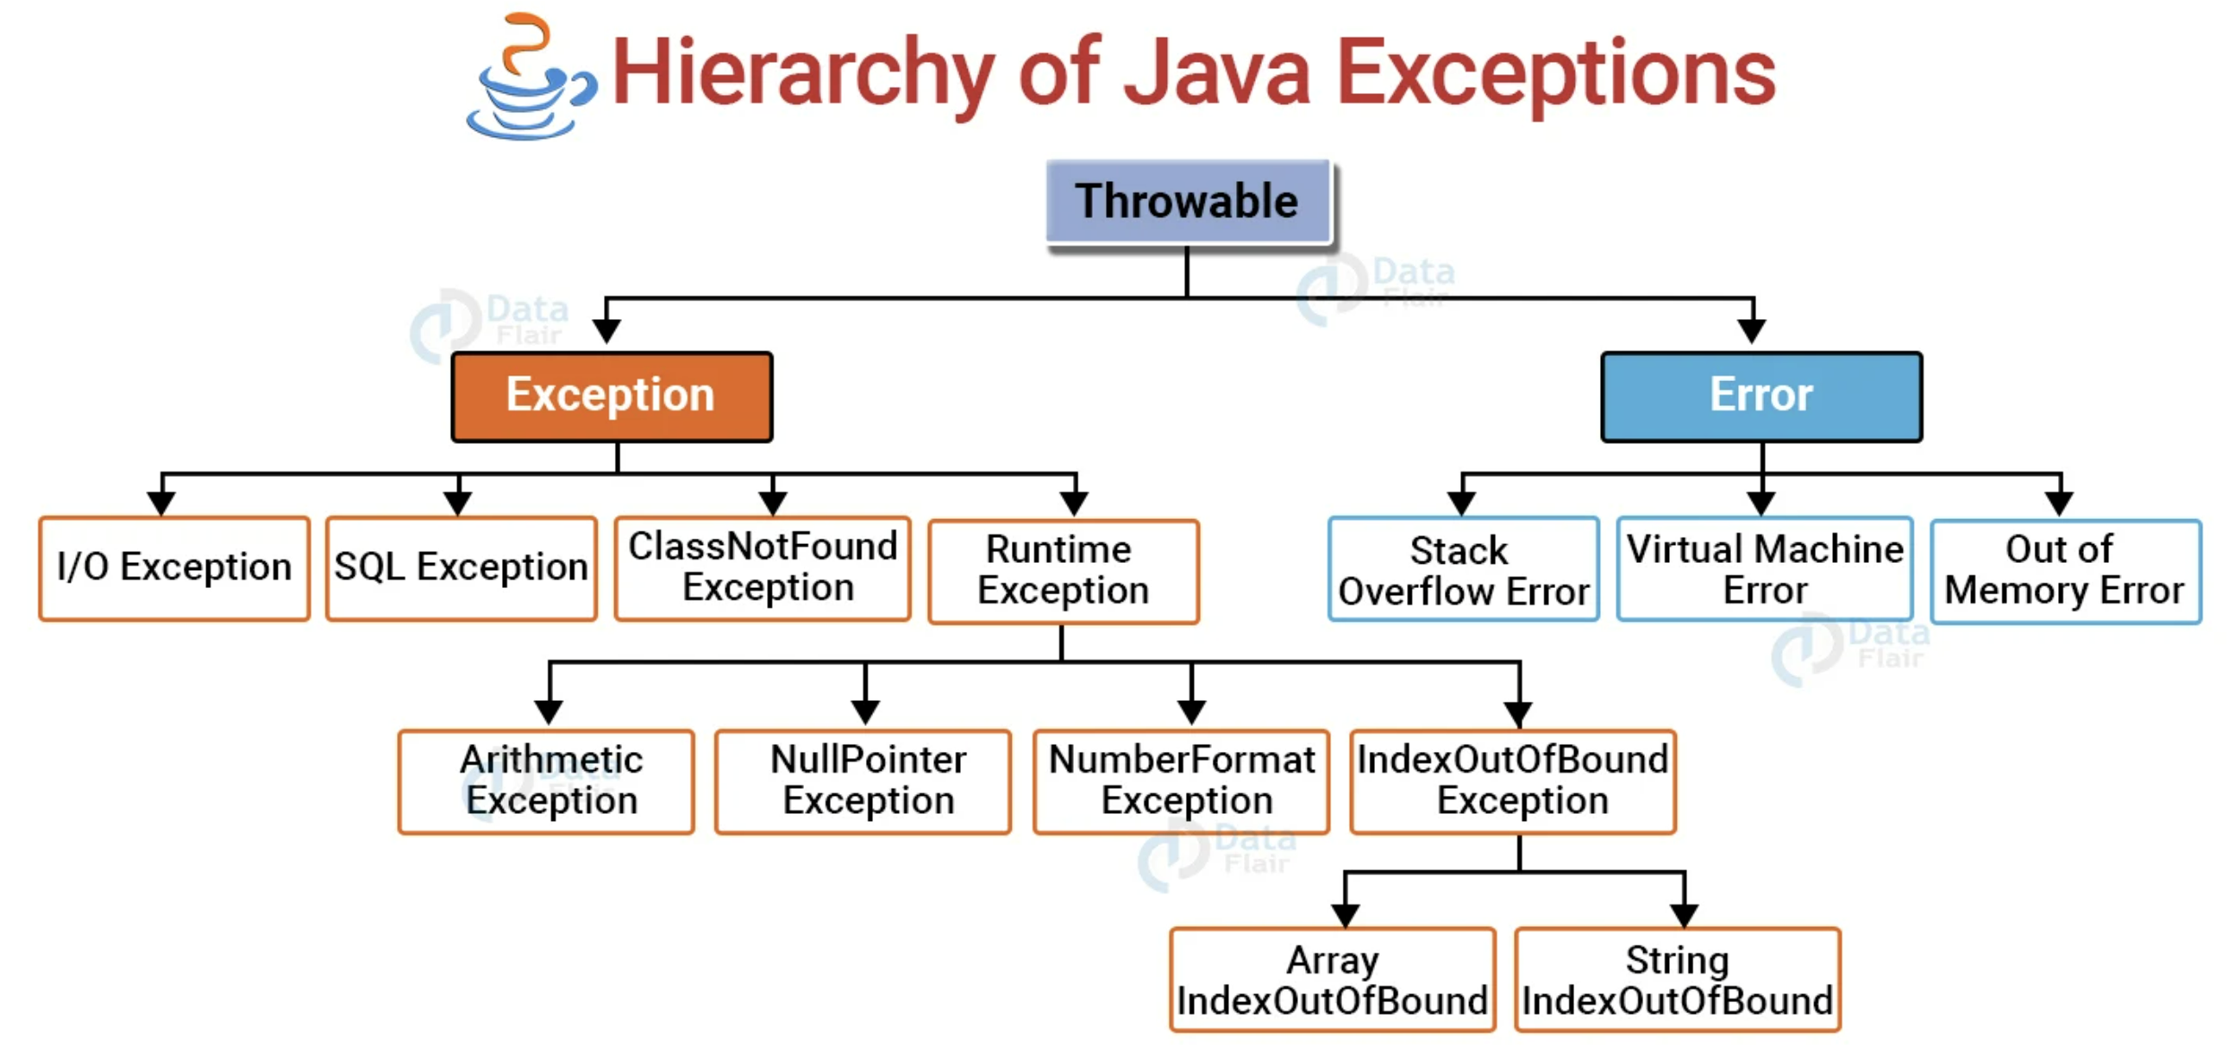
\includegraphics[width=0.9\linewidth]{exceptionhierarchy}
	\item A \textbf{checked exception} (Caught at Compile Time) must be handled either by \textbf{re-throwing} or with a try catch block, whereas an \textbf{unchecked exception} (Caught at Runtime) isn’t required to be handled.
\end{itemize}
	\centerline{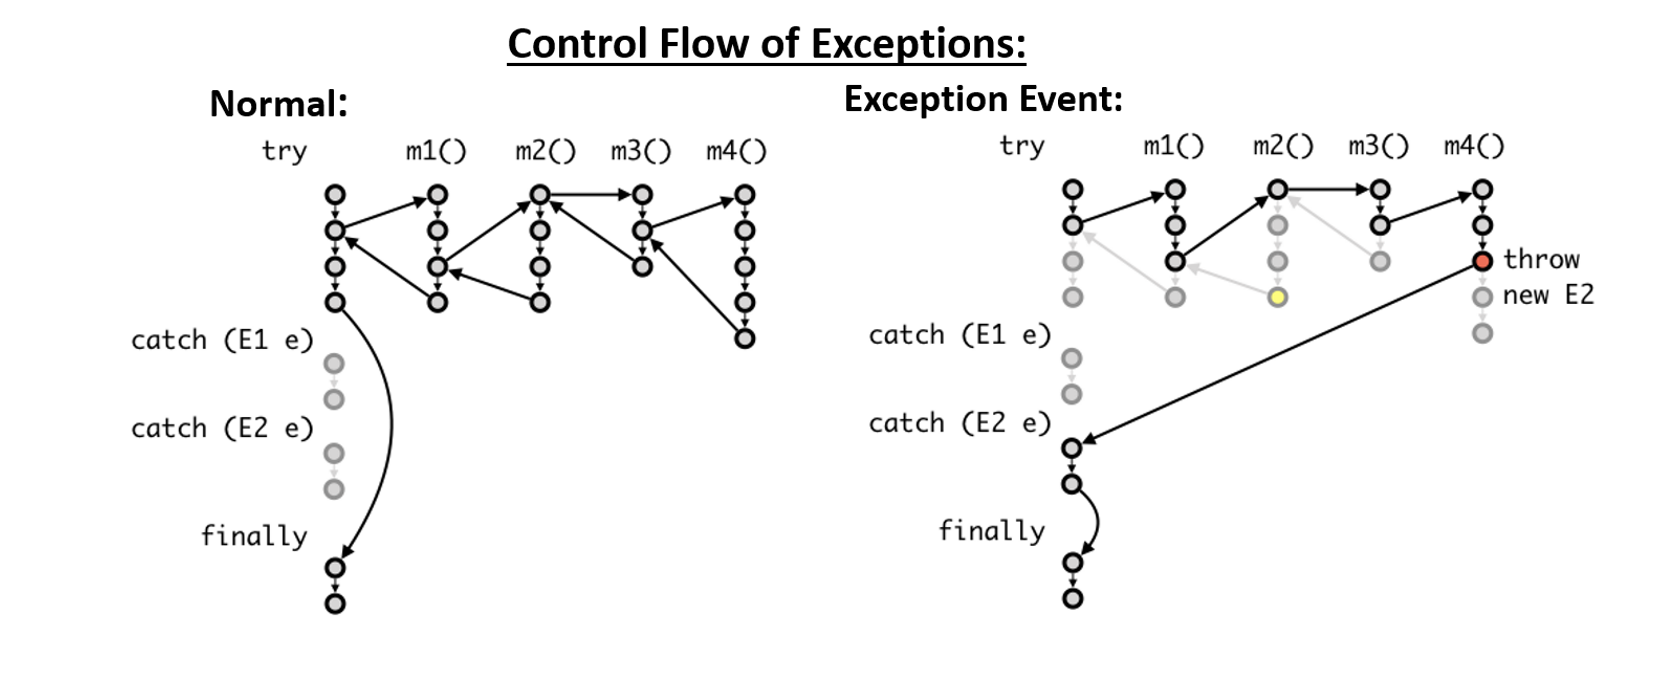
\includegraphics[width=0.9\linewidth]{exceptionevent}}



\section{Generics}
\begin{itemize}
	\item Allows classes/methods (that use reference types) to be defined without resorting to use of Object type.
	\item Ensures \textbf{type safety} $\rightarrow$ binds a generic type to a specfic type at compile time. Attempt to pass an incompatible type would lead to a compilation error.
	\item Errors will be at compile time instead of runtime.
	\item Generics are \textbf{invariant} in Java.
	\subsubsection{Generic Class:}
\begin{lstlisting}
class Pair<S extends Comparable<S>, T> implements Comparable<Pair<S, T>> {...}
class DictEntry<T> extends Pair<String, T> {...}
\end{lstlisting}

	\subsubsection{Generic Method:}
\begin{lstlisting}
// note generic goes before return type!
public static <T> boolean contains(T[] arr, T obj){...}
//to call generic method:
A.<String>contains(strArray, "hello");
\end{lstlisting}
	\item $\star$ type parameter \code{<?>} is declared before return type.
	\item note bounded type parameters. \textbf{Notes:}

\begin{lstlisting}
B implements Comparable<B>{...}
A extends B {...}
 // A <: B <: Comparable<B>
// Comparable<A> INVARIANT Comparable<B>
// Comparable<A> <: Comparable<? extends B>
\end{lstlisting}
\end{itemize}

%TYPE ERASURE --------------------------------------
\section{Type Erasure}
\begin{itemize}
	\item at compile time, type parameters are replaced by \code{Object} or the bounds (e.g. \code{T extends Comparable<T>}, \code{T} is replaced by / erasured to \code{Comparable})

\begin{lstlisting}
Integer i = new Pair<String, Integer>("x", 4).foo() //before
Integer i = (Integer) new Pair("x", 4).foo() //after
\end{lstlisting}

	\item Java Generics are not \textbf{reifiable} due to type erasure. (Reifiable type where full type information is available during run time.) 
	\item Hence, to prevent heap pollution, where Java arrays are reifiable, arrays are not generic.
\end{itemize}

\subsection{Suppress Warnings}
\begin{itemize}
	\item \code{@SupressWarnings} can only apply to declaration.
\end{itemize}

\begin{lstlisting}
@SuppressWarnings("unchecked") \\, "rawtype"
T[] a = (T[]) new Object[size];
this.array = a;
\end{lstlisting}

\subsection{Raw Types}
\begin{itemize}
	\item A generic type used without type arguments.
	\item Only acceptable as an operand of \code{instanceof}
	\item \code{@SuppressWarnings("rawtypes")} : This is when compiler is not sure if line is a type safe operation, as we are using a Raw Type (generic type w/o type arguments).
	\item The compiler cannot check e.g. if it is safe to pass an \code{Integer} to the \code{keep} method. (in case it is populated with some other type, which could e.g. cause a \code{ClassCastException} trying to cast \code{Integer} to a \code{String}. Hence, allow, but warn the programmer (unsafe). (Raw types must not be used)
\end{itemize}

\section{Wildcards}
\begin{itemize}
	\item \textbf{upper-bounded}: \code{? extends} \textbf{covariant} 
	\begin{itemize}
		\item  if \code{S <: T},  then \code{A<? extends S>} $<:$ \code{A<? extends T>}
	\end{itemize}
	\item \textbf{lower-bounded}: \code{? super} : 	\textbf{contravariant}
	\begin{itemize}
		\item if \code{S <: T},  then \code{A<? super T>} $<:$ \code{A<? super S>}
	\end{itemize}

	\item \textbf{unbounded}: \code{?}
	\begin{itemize}
		\item \code{Array<?>} is the supertype of all generic \code{Array<T>}
	\end{itemize}
\end{itemize}

\subsection{PECS Principle}
\begin{itemize}
	\item \code{PE} $\rightarrow$ If variable produces T values, use \code{List<? extends T>}
	\item \code{CS} $\rightarrow$ If variable consumes T values, use \code{List<? super T>}
	\item If both producer \& consumer $\rightarrow$ use wildcard \code{<?>}
\end{itemize}


\section{Type Inference}
\begin{itemize}
	\item Ensures \textbf{Type Safety} $\rightarrow$ compiler can ensure that \code{List<myObj>} holds objects of type \code{myObj} at compile type instead of runtime. 
	\item Type inference always chooses narrowest bound
	\item \code{<? super Integer>} $\rightarrow$ $\implies$ inferred as \code{Object} (supertype of Integer)
	\item \code{<? extends Integer>} $\rightarrow$ $\implies$ inferred as \code{Integer}

\subsubsection{Diamond Operator \code{<>}}
\begin{lstlisting}
Pair<String, Integer> p = new Pair<>();
\end{lstlisting}
	\item only for instantiating a generic type - not as a type \\
	e.g. \code{new Pair<>() //ok} \\
	\code{Pair<> p = ... //not ok}
	\item generic methods: type inference is automatic
	\item \code{A.contains()} and not \code{A.<>contains()} (no need)

\subsubsection{Constraints for Type Inference}
	\item 1. target typing $\rightarrow$ the type of expression (e.g. \code{Shape})
	\item 2. type parameter bounds $\rightarrow$ \code{<T extends GetAreable>}
	\item 3. parameter bounds \\
	$\rightarrow$ \code{Array<Circle>} $<:$ \code{Array<? extends T>}. So, \code{Circle <: T}

\begin{lstlisting}
public static <T extends GetAreable> T findLargest(Array<? extends T> array)

Shape o = A.findLargest(new Array<Circle>(0));
\end{lstlisting}

\end{itemize}









\end{multicols*}
\end{document}
